\chapter[Introduction]{Introduction}\label{chapter:introduction}

\begin{quote}\itshape
This chapter defines the robot-software synthesis problem addressed by the
thesis and explains why successful use of an existing robot interface does not
establish that an LLM can design and implement that interface. It then states
three research questions: a fixed-input comparison of LLM backbones, an
evaluation of task-grounded capability and validation design, and a matched
test of Continued Evolution in later synthesis runs. The chapter concludes by
stating the contributions, scope, and structure of the thesis.
\end{quote}

\section[Motivation]{Motivation}
\label{sec:intro-motivation}

Tool-using LLM systems can interpret instructions and compose robot operations
through an existing interface
\citep{ahn2022saycan,liang2023codeaspolicies}. However, they generally assume
that the target robot already exposes the required tool API. This assumption
leaves an upstream problem unresolved: the robot-specific software behind
those tools must still be authored.

Consider an SO-ARM101 arm described by an MJCF file containing its joints,
actuators, and motion limits. The \emph{high-level controller} selects and
sequences robot operations. It can request a Cartesian move through
\texttt{get\_ee\_pose()} and \texttt{move\_cartesian(...)}. Yet the second call
requires software that converts the requested pose into valid joint or actuator
commands. This thesis calls the reusable caller-facing contract the
\emph{robot capability interface}. Each task-neutral operation is a
\emph{capability}. The executable implementation for one robot configuration
is the \emph{robot-specific driver}.

The driver remains robot-specific even when the task is unchanged. Joint
naming, actuator semantics, units, coordinate frames, and observations vary
across configurations. Robotics frameworks therefore still require connection,
calibration, state reading, and command writing for each new platform
\citep{lerobot2026hardware,ros2control2026hardware}. Reusing a planner or learned
policy does not remove this integration requirement.

Auto-Adapter addresses this gap by making software-layer authoring part of the
LLM workflow. It receives machine-readable robot information and source-backed
target tasks with reviewed pass standards. From these inputs, it derives
reusable capabilities and measurable acceptance criteria. It then synthesises
a robot-specific driver that implements the resulting interface. A separate
high-level controller can therefore operate through task-neutral tools without
implementing robot-specific control logic.

Executable code alone cannot establish correct physical behaviour. A driver
may control the wrong joints, use incorrect units, or produce an unintended
outcome. This is an instance of the software test-oracle problem
\citep{barr2015oracle,araujo2023rasreview}. Auto-Adapter therefore separates
synthesis from behavioural evaluation. An independent \emph{Harness} owns
private validation cases, observes simulator state, and applies fixed
requirements. This evidence supports behavioural claims only under evaluated
Direct-MuJoCo conditions. It does not establish hardware performance or
sim-to-real transfer.



\section[Research Objectives]{Research Objectives}
\label{sec:research-objectives}

The aim of this thesis is to develop and evaluate Auto-Adapter as a framework
for automating robot-software synthesis. Auto-Adapter starts from a
machine-readable robot description and a source-backed collection of target
tasks with reviewed pass standards. It constructs the required software layer
by designing a reusable robot capability interface and synthesising the
robot-specific driver that implements it. The interface exposes task-neutral
robot operations as tools to a separate high-level controller. The driver
translates each requested operation into commands for the declared robot
configuration. An independent Harness evaluates the resulting behaviour
against fixed requirements under controlled Direct-MuJoCo conditions.

This aim is expressed through three research questions:

\begin{enumerate}
    \item \textbf{RQ1---End-to-end robot-software synthesis and downstream use.}

    To what extent can Auto-Adapter produce robot-specific drivers that pass
    independent behavioural validation and support downstream embodied-task
    completion by a separate high-level controller?

    \item \textbf{RQ2---Task-grounded capability and validation design.}

    \textbf{(a)} To what extent can an LLM derive five to ten reusable
    capabilities from at least twenty source-backed tasks without receiving a
    pre-authored capability catalogue or task-to-capability mapping?

    \textbf{(b)} Can the LLM formulate source-grounded capability-level pass
    criteria from reviewed task-level standards without human predefinition at
    the capability level, and can an implementation-blind Independent
    Validation Compiler audit and compile those criteria into private
    executable validation without weakening their source obligations?

    \item \textbf{RQ3---Continued Evolution in later driver synthesis.}

    With the robot, LLM backbone, fixed capability-and-validation inputs,
    generation condition, evaluation protocol, and resource budget held
    constant, what effect, if any, does access to human-reviewed Experience
    derived from completed terminal runs have on later driver-synthesis
    outcomes relative to matched runs without that Experience?
\end{enumerate}

\begin{figure}[htbp]
  \centering
  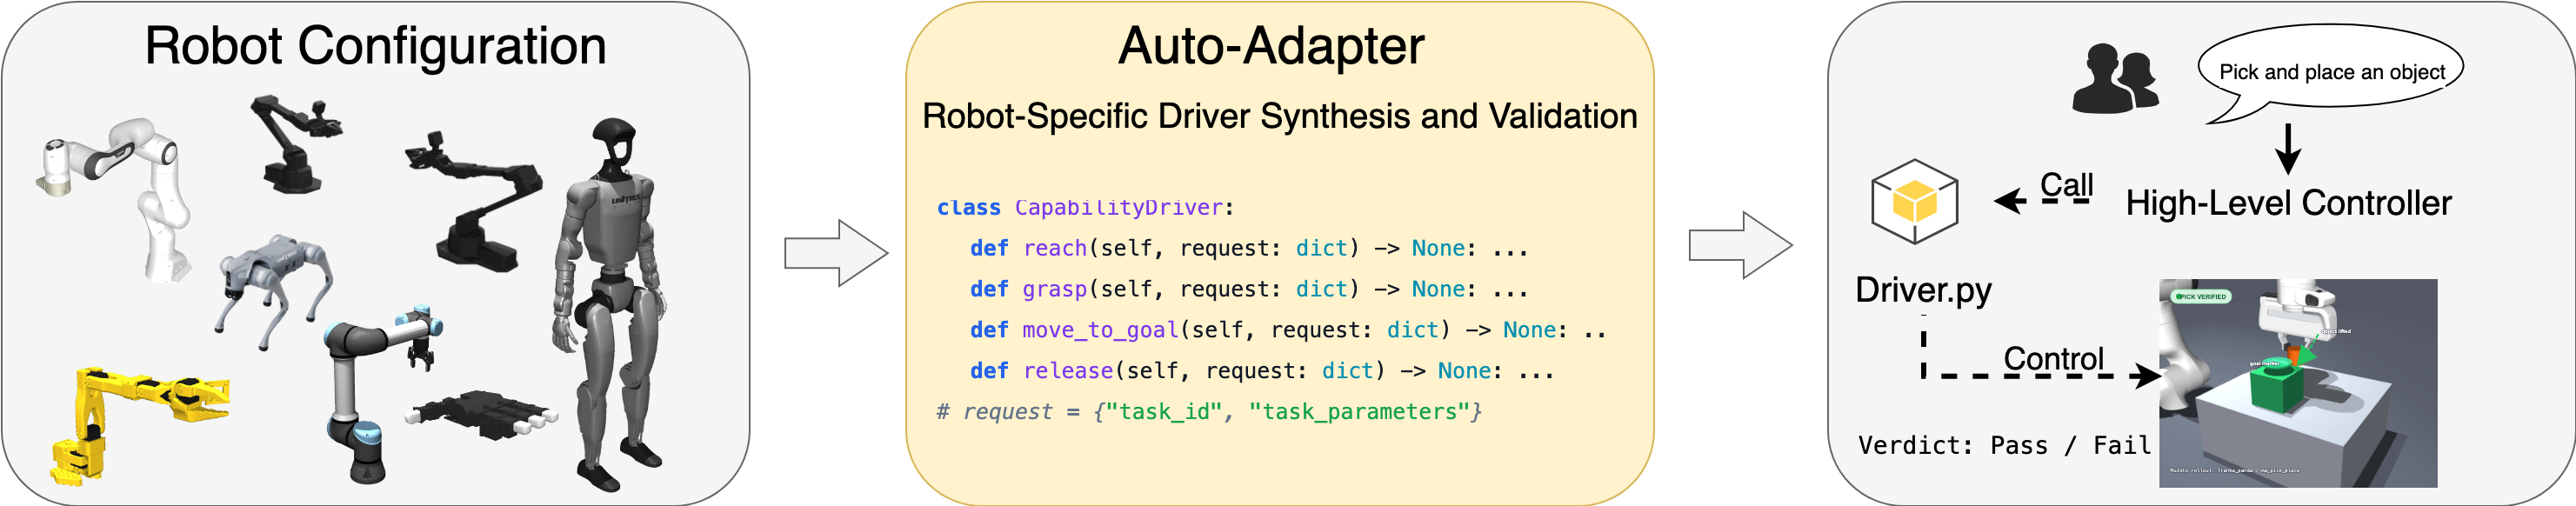
\includegraphics[width=\linewidth]{assets/abstract.drawio.png}
  \caption{Conceptual role of Auto-Adapter. The framework designs a reusable
  robot capability interface, synthesises a robot-specific driver that implements
  it, and independently evaluates the driver's behaviour under controlled
  Direct-MuJoCo conditions.}
  \label{fig:introduction-auto-adapter-role}
\end{figure}

\label{sec:intro-scope}
These questions concern the declared LLM endpoints, robot configurations,
tasks, generation conditions, and Direct-MuJoCo evaluation protocols. The
selected robot configurations are experimental cases rather than a
representative sample from which morphology effects can be estimated. The
resulting evidence does not establish real-SDK fidelity, hardware performance
or safety, sim-to-real transfer, physical validation of unselected tasks,
downstream high-level-controller performance, universal model or robot
superiority, autonomous self-improvement, or generalisation beyond the
evaluated conditions. The following section translates the questions into
three controlled experiments.


\section[Research Experiments]{Research Experiments}
\label{sec:research-experiments}
\label{sec:research-programme}

The empirical programme contains three experiments with distinct inputs and
evidence boundaries. Their numbering follows the analytical questions and
chapter order rather than the runtime production order. Experiment~1 consumes
prior-designed and sealed capability-and-validation inputs. Experiment~2
evaluates the upstream process used to create that type of input, whose
accepted outputs must be fixed before Experiment~1 begins. Experiment~3 can
affect only later runs after terminal evidence has been reviewed.

\begin{enumerate}[leftmargin=*,itemsep=1em]
    \item \textbf{Experiment 1---Fixed-input comparison of LLM backbones for
    robot-specific driver synthesis (AutoAdapter-Bench, Chapter~3).}

    Experiment~1 compares seven LLM backbones across five robot configurations,
    two generation conditions, and three independent replicates, producing a
    primary matrix of 210 experimental cells. For each robot, one public
    capability interface, its capability-level pass standards, and the complete
    private validation suite are fixed across all backbones, conditions,
    replicates, and submitted attempts. The skeleton-assisted condition may
    inspect the trusted implementation skeleton, whereas the from-scratch
    condition may not. Each cell begins with empty Experience and permits at
    most three submitted driver attempts.

    The experiment reports initial and final driver-validation outcomes, Repair
    recovery, failure classes, model calls, token use, cost, and wall-clock
    time. It begins with driver study and generation and stops at the terminal
    Harness verdict. It does not run Task-Grounded Capability Design, the
    Independent Validation Compiler, a high-level controller, or Evolution.

    \item \textbf{Experiment 2---Task-grounded capability and validation
    design (Chapter~4).}

    Experiment~2 evaluates the upstream production of the capability and
    validation inputs consumed by fixed-input driver synthesis. The first part
    examines whether an LLM can derive five to ten reusable capabilities from
    at least twenty source-backed tasks without receiving a pre-authored
    catalogue or task-to-capability mapping. The analysis distinguishes
    complete task coverage from evidence that the grouping represents shared
    robot effects rather than renamed task-specific programs.

    The second part examines whether the LLM can formulate measurable
    capability-level pass criteria that preserve the obligations in the
    reviewed task-level standards. An implementation-blind Independent
    Validation Compiler audits those criteria without access to a candidate
    driver, synthesis trace, Repair history, or validation result, and binds
    accepted criteria to private MuJoCo cases, measurements, resets, and
    guards. Compilation success is reported separately from Harness calibration
    and false-success checks. The Independent Validation Compiler does not issue
    final driver verdicts, and a generated or compilable criterion is not
    treated by itself as reliable validation.

    \item \textbf{Experiment 3---Matched evaluation of Continued Evolution
    (Chapter~5).}

    After an eligible run reaches a terminal verdict, Evolution reads a bounded
    projection of its terminal report and proposes either one candidate
    Experience record or an explicit \texttt{no-reusable-lesson} outcome. Human
    review determines whether a proposal is accepted or rejected. Only
    accepted, public, non-private content may enter a versioned Experience
    snapshot supplied to a later run.

    Evolution cannot alter the originating driver, validation suite, criterion,
    Repair decision, retry decision, run inputs, or terminal verdict.
    Experiment~3 compares later driver-synthesis runs supplied with reviewed
    Experience against matched runs without Experience. The comparison reports
    driver-validation, Repair, failure, model-use, cost, and time outcomes under
    the matching factors fixed prospectively for Experiment~3. The existence of
    an Evolution proposal is not itself treated as evidence of improvement.
\end{enumerate}

Together, the experiments separate three claims: whether different LLM
backbones can implement a fixed robot interface, whether the interface and its
validation can be designed from source-backed tasks, and whether reviewed
evidence from completed runs changes later synthesis outcomes. The following
section states the contributions that this evidence is designed to support.


\section[Contributions]{Contributions}
\label{sec:intro-contributions}

This thesis makes three scientific contributions and three bounded,
industry-relevant contributions. The scientific contributions concern how
LLM-based robot-software production, use, validation, and adaptation can be
studied as separate empirical objects. The industry-relevant contributions
concern the experimental infrastructure and decision evidence made available
within the declared Direct-MuJoCo scope.

The scientific contributions are as follows:

\begin{enumerate}[leftmargin=*,itemsep=0.8em]

  \item \textbf{A layer-separated benchmark of LLMs as producers and users of
  robot software.}

  Existing evaluations examine supplied-interface use, task-conditioned robot
  programme generation, or coding-agent performance under robot tests
  \citep{liang2023codeaspolicies,hu2024codebotler,fu2026capx}. These outcomes do
  not by themselves reveal whether a model can implement a reusable robot
  interface and then use a fixed implementation. AutoAdapter-Bench addresses
  this measurement gap through two non-interchangeable model roles.
  Experiment~1 evaluates whether a Producer backbone can synthesise a
  robot-specific driver that implements a fixed capability interface. The
  separately scoped B2 extension evaluates whether a high-level-controller
  backbone can complete tasks through an already fixed and validated
  driver--capability-interface--adapter stack. The tracks use different
  experimental units, verdicts, and resource measures, and are therefore
  reported separately rather than collapsed into an aggregate model score or
  ranking.

  \item \textbf{An evidence-governed synthesis lifecycle for model-authored
  robot capabilities and controlled adaptation.}

  Auto-Adapter formulates robot-software synthesis as a staged lifecycle rather
  than a single prompt-to-code event. Task-Grounded Capability Design makes
  capability-layer design a first-class empirical object by deriving reusable
  capability contracts from source-backed tasks. Driver Synthesis attempts to
  implement those contracts; bounded Repair revises the current driver using
  permitted execution evidence; and terminal Evolution may propose
  human-reviewed Experience for a prospectively matched later run. Each stage
  has an explicit information and evidence boundary. This makes capability
  abstraction, implementation, within-run correction, and cross-run evidence
  reuse independently observable while preventing later Experience from
  changing the run that produced it.

  \item \textbf{An implementation-blind, physics-grounded test-oracle
  architecture for generated robot software.}

  Model-authored capability-level pass criteria are derived from reviewed
  source obligations, but an Independent Validation Compiler audits source
  preservation and binds accepted criteria to private executable cases without
  access to the candidate implementation. The trusted Harness then owns
  simulator-state observations, physical-integrity guards, aggregation, and the
  final verdict. This architecture prevents the code generator from determining
  its own correctness and distinguishes structural validity or successful
  compilation from demonstrated actuator-mediated behavioural validity under
  the declared Direct-MuJoCo conditions.

\end{enumerate}

Within the declared Direct-MuJoCo scope, the bounded industry-relevant
contributions are as follows:

\begin{enumerate}[leftmargin=*,itemsep=0.8em]

  \item \textbf{A bounded and inspectable workflow for LLM-assisted robot
  integration.}

  A general-purpose coding agent can generate candidate robot-integration code,
  but code generation alone does not define the robot contract, constrain
  revision, account for resource use, or establish behavioural acceptance.
  Auto-Adapter fixes the robot-facing inputs and caller-facing capability
  interface for each comparison; bounds model interaction, public probes,
  submitted drivers, and Repair; records model identity, calls, tokens, cost,
  time, revisions, and observable actions; and assigns the final verdict to the
  trusted Harness. This converts open-ended code generation into a repeatable
  experimental workflow whose inputs, resource use, revisions, physical
  observations, and acceptance evidence can be inspected.

  \item \textbf{A reusable experimental substrate for embodied-AI research and
  development.}

  Embodied-AI studies commonly require working robot-facing software before
  high-level controllers can be evaluated. For each admitted experimental
  stack, Auto-Adapter exposes a stable capability interface backed by a driver
  that has passed independent Direct-MuJoCo capability validation. Researchers
  can therefore hold the low-level robot integration fixed while comparing
  high-level-controller backbones against the same callable boundary. This
  provides a reusable substrate for controlled task-level experiments without
  claiming universal interoperability, real-SDK portability, hardware
  readiness, or a measured reduction in engineering effort.

  \item \textbf{A resource-accounted basis for role-specific LLM selection.}

  The Producer track records driver-validation outcomes together with Repair,
  failure, model-call, token, monetary-cost, and timing measures. The
  capability-interface-use track separately records task-level Harness
  verdicts, invalid controller outputs, model and capability calls, tokens,
  cost, simulation time, and wall time. These records support two distinct
  engineering decisions: which Producer backbone and generation condition to
  use for fixed-input driver synthesis, and which controller backbone to use
  after the robot-facing stack has been fixed. The resulting evidence remains
  conditional on the evaluated configurations rather than constituting a
  universal model ranking, production total-cost estimate, or general
  procurement recommendation.

\end{enumerate}

These contributions apply only to the declared tasks, robot configurations,
generation conditions, model endpoints, and Direct-MuJoCo evaluation
protocols. They do not establish compliance with an industry standard,
industrial certification, real-SDK fidelity, hardware safety, sim-to-real
transfer, reduced real-world integration time or cost, production reliability,
security containment, universal robot or model superiority, or a causal
morphology effect.

Experiment~1 provides evidence only about fixed-input robot-specific driver
synthesis. B2 provides separate capability-interface-use evidence only for its
fixed validated stacks, selected tasks, ReCAP controller, and declared
backbones; it is not Experiment~2 or RQ2, does not show that its reference
drivers were synthesised, and does not establish that ReCAP is superior to
another controller. Experiment~2 cannot treat a generated or compilable
criterion as reliable without its declared audit, calibration, and
false-success evidence. Experiment~3 can support an Experience effect only
through prospectively matched later runs and does not establish autonomous or
same-run self-improvement.


\section[Thesis Structure]{Thesis Structure}
\label{sec:intro-structure}

The structure of this thesis is organised as follows:

\begin{itemize}[leftmargin=*,itemsep=0.7em]

  \item Chapter~2---Background and Literature Review. This chapter defines the
  relationship between high-level controllers, robot capability interfaces,
  and robot-specific drivers. It reviews LLM tool use, robot-software
  synthesis, task-grounded abstraction, independent validation, iterative
  Repair, and cross-run evidence reuse. It concludes by identifying the
  assumptions that reusable capability interfaces, robot-specific
  implementations, capability-level pass criteria, and executable validation
  already exist.

  \item Chapter~3---AutoAdapter-Bench: Fixed-Input Comparison of LLM Backbones
  in Robot-Specific Driver Synthesis. This chapter presents Experiment~1. It
  compares seven LLM backbones across five robot configurations under
  skeleton-assisted and from-scratch generation. For each robot, the capability
  interface, pass standards, complete private validation suite, Harness rules,
  and resource budget remain fixed. The chapter reports initial and final
  validation, Repair, failure, model-use, cost, and time outcomes across the
  210-cell primary matrix.

  \item Chapter~4---Task-Grounded Capability and Validation Design. This
  chapter presents Experiment~2. It first evaluates whether an LLM can derive
  five to ten reusable capabilities from at least twenty source-backed tasks
  without a pre-authored catalogue or mapping. It then evaluates whether the
  LLM can formulate source-preserving capability-level pass criteria that an
  implementation-blind Independent Validation Compiler can audit and compile.
  Harness calibration and false-success evidence are reported separately from
  compilation success. Although the chapter follows Experiment~1 in the thesis,
  accepted outputs of this upstream process must be fixed before
  Experiment~1 begins.

  \item Chapter~5---Continued Evolution: Matched Evaluation of Reviewed
  Experience. This chapter presents Experiment~3. It describes how terminal
  reports are projected into bounded Evolution proposals, how human review
  determines which proposals become Experience, and how accepted Experience is
  versioned for later runs. It then compares matched driver-synthesis runs with
  and without reviewed Experience. Evolution cannot alter the run from which
  its evidence was derived.

  \item Chapter~6---Conclusion and Future Work. The final chapter
  answers the research questions in order and synthesises the evidence from
  Chapters~3--5. It relates the findings to the scientific and bounded industry
  contributions, states the limits of the Direct-MuJoCo evaluation, and
  identifies future work arising from those limits.

\end{itemize}
